
% VLDB template version of 2020-08-03 enhances the ACM template, version 1.7.0:
% https://www.acm.org/publications/proceedings-template
% The ACM Latex guide provides further information about the ACM template

\documentclass[sigconf, nonacm]{acmart}
\usepackage{enumitem}
% pipeline_figure.pdf has a full-page bounding box (~87% of textheight when scaled
% to textwidth). Default \topfraction=0.7 rejects it every page and defers it to
% the end of the document. Raise the limit so tall figures can be placed at [t].
\renewcommand{\topfraction}{0.95}
\renewcommand{\floatpagefraction}{0.85}
\renewcommand{\dbltopfraction}{0.95}     % for figure* in two-column
\renewcommand{\dblfloatpagefraction}{0.85}

%% The following content must be adapted for the final version
% paper-specific
\newcommand\vldbdoi{XX.XX/XXX.XX}
\newcommand\vldbpages{XXX-XXX}
% issue-specific
\newcommand\vldbvolume{14}
\newcommand\vldbissue{1}
\newcommand\vldbyear{2020}
% should be fine as it is
\newcommand\vldbauthors{\authors}
\newcommand\vldbtitle{\shorttitle} 
% leave empty if no availability url should be set
\newcommand\vldbavailabilityurl{URL_TO_YOUR_ARTIFACTS}
% whether page numbers should be shown or not, use 'plain' for review versions, 'empty' for camera ready
\newcommand\vldbpagestyle{plain} 

\begin{document}
\title{LLM-Guided ANN Index Optimization for Efficient Human-Object Interaction Retrieval}

%%
%% The "author" command and its associated commands are used to define the authors and their affiliations.
\author{Shahrzad Esmat}
\affiliation{%
  \institution{Iowa State University}
  \city{Ames}
  \state{Iowa}
  \country{USA}
}
\email{sesmat@iastate.edu}

\author{Chaunte W. Lacewell}
\affiliation{%
  \institution{Intel Corporation}
  \country{USA}
}
\email{chaunte.w.lacewell@intel.com}

\author{Sameh Gobriel}
\affiliation{%
  \institution{Intel Corporation}
  \country{USA}
}
\email{sameh.gobriel@intel.com}

\author{Nilesh Jain}
\affiliation{%
  \institution{Intel Corporation}
  \country{USA}
}
\email{nilesh.jain@intel.com}

\author{Ali Jannesari}
\affiliation{%
  \institution{Iowa State University}
  \city{Ames}
  \state{Iowa}
  \country{USA}
}
\email{jannesar@iastate.edu}

%%
%% The abstract is a short summary of the work to be presented in the
%% article.
\begin{abstract}
Human-Object Interaction (HOI) benchmarks have been exclusively exploited for detection --- predicting bounding boxes and interaction labels given an image. Their rich compositional semantics make them equally compelling for text-query image retrieval, yet no prior work has explored this direction. We introduce the first retrieval benchmark derived from HICO-DET (47,776 images, 600 HOI categories) and propose a two-stage pipeline in which CLIP ViT-L/14 text embeddings drive Approximate Nearest Neighbor (ANN) search over a VDMS vector database, followed by zero-cost DINOv2 ViT-L/14-reg4 visual reranking over the top-$k$ candidate pool --- requiring only one ANN index at deployment. DINOv2 reranking improves mAP by 3.65 percentage points ($+$15.2\%) over CLIP-only retrieval at under 1\% additional query latency. To jointly optimize retrieval accuracy and throughput --- measured as Score $=$ mAP $\times$ QPS --- we present the first LLM agent applied to vector database ANN index hyperparameter optimization, iteratively reasoning over observed outcomes to propose engine type, graph connectivity, search depth, candidate pool size, and fusion weight. Our optimized pipeline achieves Score $= 4.34$, a $2.5\times$ improvement over the CLIP FaissFlat baseline and $13.6\times$ over brute-force CLIP$+$DINOv2 reranking. The LLM agent reaches competitive performance within 5 iterations --- a level requiring 9 iterations for Optuna TPE and 28 for Random Search --- demonstrating substantially superior sample efficiency.
\end{abstract}

\maketitle

%%% do not modify the following VLDB block %%
%%% VLDB block start %%%
\pagestyle{\vldbpagestyle}
\begingroup\small\noindent\raggedright\textbf{PVLDB Reference Format:}\\
\vldbauthors. \vldbtitle. PVLDB, \vldbvolume(\vldbissue): \vldbpages, \vldbyear.\\
\href{https://doi.org/\vldbdoi}{doi:\vldbdoi}
\endgroup
\begingroup
\renewcommand\thefootnote{}\footnote{\noindent
This work is licensed under the Creative Commons BY-NC-ND 4.0 International License. Visit \url{https://creativecommons.org/licenses/by-nc-nd/4.0/} to view a copy of this license. For any use beyond those covered by this license, obtain permission by emailing \href{mailto:info@vldb.org}{info@vldb.org}. Copyright is held by the owner/author(s). Publication rights licensed to the VLDB Endowment. \\
\raggedright Proceedings of the VLDB Endowment, Vol. \vldbvolume, No. \vldbissue\ %
ISSN 2150-8097. \\
\href{https://doi.org/\vldbdoi}{doi:\vldbdoi} \\
}\addtocounter{footnote}{-1}\endgroup
%%% VLDB block end %%%

%%% do not modify the following VLDB block %%
%%% VLDB block start %%%
\ifdefempty{\vldbavailabilityurl}{}{
\vspace{.3cm}
\begingroup\small\noindent\raggedright\textbf{PVLDB Artifact Availability:}\\
The source code, data, and/or other artifacts have been made available at \url{\vldbavailabilityurl}.
\endgroup
}
%%% VLDB block end %%%

\section{Introduction}
\label{sec:intro}

The rapid adoption of large-scale vision-language foundation models has elevated image retrieval
from a narrow computer vision task to a central infrastructure challenge.
Models such as CLIP~\cite{radford2021clip} and DINOv2~\cite{oquab2024dinov2} produce rich
semantic embeddings that encode not only visual appearance but also object identity and
compositional scene understanding.
Deployed over vector databases with Approximate Nearest Neighbor (ANN) indexing, these embeddings
enable sub-second similarity search over collections of tens of millions of images --- a
capability now integral to e-commerce product discovery, medical image retrieval, and multimodal
AI assistants~\cite{pan2023vdms,aguerrebere2023locally}.
Yet while the database community has invested heavily in the efficiency of ANN
search~\cite{malkov2018hnsw,johnson2019billion}, far less attention has been paid to the
depth of semantic expressiveness that retrieval benchmarks actually demand.
Most existing benchmarks test retrieval of visually similar images or single objects; none
probe whether a system can distinguish 600 fine-grained human activities from natural language.

Human-Object Interaction (HOI) recognition captures one of the richest forms of compositional
visual semantics available in any public benchmark.
HICO-DET~\cite{chao2018hico} annotates 47{,}776 images across 600 fine-grained
interaction categories structured as \textit{verb--object} pairs spanning 80 object
classes and 117 action verbs.
Despite this semantic richness, every published use of HICO-DET has been restricted to the
\emph{detection} paradigm: predicting bounding boxes and interaction class labels from a given
image.
The \emph{retrieval} direction --- in which a natural-language query such as
\emph{``a person riding a horse''} should rank all 47{,}776 images by relevance --- has never been
explored.
This is a significant missed opportunity: the same compositional label structure that makes
HOI detection challenging makes HOI retrieval a uniquely demanding test of cross-modal alignment
between language and visual content, providing a far more discriminative evaluation signal
than scene-level or object-level benchmarks.

Establishing HOI retrieval as a benchmark task immediately surfaces two open technical problems.
First, practitioners must decide between two query modalities: a natural-language description
or a reference image.
The relative merits of text versus image queries on a compositionally structured dataset have
not been quantified, and the underlying geometric reason for any observed difference has not
been articulated.
Second, once embeddings are stored in a vector database, the ANN index
hyperparameters --- graph connectivity ($M$), search depth (\textit{efSearch}), candidate
pool size ($k$), and the fusion weight $\alpha$ blending ANN retrieval scores with visual
reranking signals --- jointly determine the accuracy--throughput trade-off in ways that
interact non-linearly and depend on the data distribution.
Current practice resorts to grid search or random search: \emph{blind} procedures that
evaluate configurations independently of all previously measured outcomes.
As vector database collections scale to tens of millions of vectors, this sample-inefficient
approach wastes substantial compute and fails to exploit the structured, measurable feedback
that each evaluated configuration already provides.

We address both problems with a unified system.
For retrieval, we propose a two-stage pipeline: in the first stage, CLIP ViT-L/14 text
embeddings drive ANN search over a VDMS vector database~\cite{pan2023vdms}, returning a
ranked candidate pool; in the second stage, DINOv2 ViT-L/14-reg4 visual embeddings rerank
the candidate pool using a weighted fusion of normalized distances --- requiring only
\emph{one} ANN index at deployment, with zero additional indexing cost for the reranker.
For modality selection, we show geometrically that a CLIP text embedding lies at the
\emph{semantic centroid} of all images sharing a given HOI category, while a reference image
is a single noisy point displaced from that centroid in the same embedding space --- a
structural difference that predicts a systematic mAP advantage for text queries on
compositionally structured datasets such as HICO-DET.
For hyperparameter optimization, we present an LLM agent that, at each iteration, observes
the measured Score ($= \text{mAP} \times \text{QPS}$) of every previously evaluated
configuration and reasons over the full history to propose the next configuration --- a
strategy fundamentally different from blind grid and random search because it conditions
each new proposal on empirical outcomes.

\smallskip
\noindent\textbf{Contributions.} This paper makes four contributions:

\begin{itemize}
  \item \textbf{The first HOI retrieval benchmark.}
    We introduce a text-query image retrieval benchmark derived from HICO-DET
    (47{,}776 images, 600 HOI categories), including ground-truth construction,
    evaluation protocol, and baselines that the community can build upon.

  \item \textbf{A deployment-efficient two-stage retrieval pipeline.}
    We propose combining CLIP ViT-L/14 ANN retrieval with zero-index-cost
    DINOv2 ViT-L/14-reg4 visual reranking, achieving a $+$3.65 percentage-point
    mAP improvement ($+$15.2\% relative) at under 1\% additional query latency
    over ANN-only retrieval --- requiring only a single index at deployment.

  \item \textbf{A geometric explanation of text query superiority.}
    We formally characterize why text queries outperform image queries on HOI
    retrieval by grounding the result in the centroid geometry of CLIP's joint
    vision-language embedding space: a text embedding is the semantic centroid
    of its category, while a reference image is a single, noisy sample displaced
    from that centroid.

  \item \textbf{The first LLM agent for ANN index hyperparameter optimization.}
    Our agent iteratively reasons over measured outcomes to select engine type,
    graph connectivity, search depth, candidate pool size, and fusion weight,
    reaching competitive performance within 5 iterations --- a level that requires
    9 iterations for Optuna TPE and 28 for Random Search.
    The optimized pipeline achieves Score $= 4.34$ ($\text{mAP} \times \text{QPS}$),
    a $2.5\times$ improvement over the CLIP FaissFlat baseline and $13.6\times$
    over brute-force CLIP$+$DINOv2 reranking~\cite{wei2023uniir}.
\end{itemize}

\smallskip
The remainder of this paper is organized as follows.
Section~\ref{sec:related} reviews related work on HOI understanding, image retrieval,
vector database systems, and hyperparameter optimization.
Section~\ref{sec:benchmark} describes the construction of the HICO-DET retrieval benchmark.
Section~\ref{sec:pipeline} presents the two-stage retrieval pipeline and the embedding
geometry analysis.
Section~\ref{sec:optimizer} details the LLM-guided ANN hyperparameter optimizer.
Section~\ref{sec:experiments} reports experimental results and ablations.
Section~\ref{sec:conclusion} concludes.

\section{Related Work}
\label{sec:related}

\subsection{Human-Object Interaction Detection}
HOI detection has been studied extensively since the introduction of HICO-DET~\cite{chao2018hico},
which defined the two-stage paradigm of detecting human--object pairs and classifying their
interactions across 600 fine-grained categories.
Early approaches used instance-centric attention to model spatial and appearance relationships
between detected instances~\cite{gao2018ican}.
The adoption of transformer architectures enabled end-to-end
detection~\cite{kim2021hotr,zhang2021cdn}, and subsequent work leveraged vision-language
pre-training to transfer interaction semantics from large-scale
models~\cite{liao2022genvlkt}.
Despite sustained progress, every published use of HICO-DET is restricted to the detection
paradigm --- predicting bounding boxes and interaction labels from a given image.
We identify and fill the orthogonal \emph{retrieval} direction: given a natural-language
query, rank all images by HOI relevance.

\subsection{Cross-Modal Image Retrieval}
Early text-image retrieval research established benchmark datasets using caption
annotations~\cite{young2014flickr30k,lin2014coco} and proposed embedding losses designed to
bring matching (image, caption) pairs close in a shared
space~\cite{faghri2018vsepp}.
The landscape changed fundamentally with CLIP~\cite{radford2021clip}, whose joint
vision-language embedding enables zero-shot retrieval across diverse domains without
task-specific fine-tuning.
BLIP-2~\cite{li2023blip2} extended this paradigm by bridging frozen visual encoders and
large language models via a lightweight querying transformer, achieving strong generalization
with substantially fewer trainable parameters.
UniIR~\cite{wei2023uniir}, an ECCV 2024 Oral, unified eight multimodal retrieval tasks within
a single model and constructed the M-BEIR benchmark spanning 1.5M queries over 10 datasets;
we adopt UniIR as our primary baseline.
No prior work has constructed a retrieval benchmark from HOI annotations or analyzed
the relative merits of text versus image queries on compositionally structured datasets.
We fill both gaps: we introduce the first HOI retrieval benchmark and provide a principled
geometric explanation of why text queries are better suited to this task.

\subsection{Approximate Nearest Neighbor Search and Vector Databases}
ANN index research has produced a rich family of scalable methods: graph-based indices
(HNSW~\cite{malkov2018hnsw}), inverted file structures combined with product
quantization~\cite{jegou2011pq}, and GPU-accelerated flat search~\cite{johnson2019billion}.
Systematic benchmarking in ANN-Benchmarks~\cite{aumuller2020ann} and the NeurIPS 2021
billion-scale competition~\cite{simhadri2022neurips} characterize the accuracy--throughput
Pareto frontier across these methods and datasets.
Purpose-built vector database management systems such as Milvus~\cite{wang2021milvus} and
VDMS~\cite{pan2023vdms} integrate ANN indexing with metadata management and production-grade
data persistence, enabling efficient multimodal workloads.
Despite this rich infrastructure, index configuration --- choosing the engine type, graph
connectivity, search depth, and candidate pool size for a given embedding distribution and
throughput target --- is universally left to blind grid or random search.
We replace these procedures with an LLM agent that reasons over all previously measured
outcomes to propose the next configuration.

\subsection{Hyperparameter Optimization}
Classical HPO methods range from grid and random search~\cite{bergstra2012random} --- the
latter empirically superior in high-dimensional spaces --- to Gaussian-process-based Bayesian
optimization~\cite{snoek2012bayesian}, bandit-based methods such as
Hyperband~\cite{li2018hyperband}, and hybrid approaches such as BOHB~\cite{falkner2018bohb}
that combine kernel density estimation with successive halving.
Automated machine learning frameworks such as Auto-sklearn~\cite{feurer2015autosklearn}
apply these methods to joint algorithm selection and hyperparameter configuration.
A key limitation of classical HPO for ANN index selection is that the search space is
\emph{mixed-type}: it includes discrete engine choices (HNSW vs.\ IVFFlat), integer
parameters ($M$, \textit{efSearch}, \textit{nlist}, $k$), and continuous parameters
($\alpha$), with structural dependencies between parameters and engine choice.
Gaussian process surrogates assume stationarity over a continuous space, making them poorly
suited to this setting; Bayesian methods also typically require warm-start priors that are
unavailable for new embedding modalities.
Tree-structured Parzen Estimators (TPE), as implemented in Optuna~\cite{akiba2019optuna},
handle mixed-type spaces more gracefully by modeling the density of good and bad
configurations separately, but they treat each parameter independently and cannot exploit
architectural knowledge about ANN indices (e.g., that $M$ and \textit{efSearch} must be
co-tuned, or that IVFFlat is preferable when $n$-probe covers a large fraction of the
cluster count).

\subsection{LLM Agents for Optimization}
Recent work has demonstrated that large language models can act as black-box optimizers by
iteratively proposing candidate solutions and refining them based on observed
outcomes~\cite{yang2024opro}.
OPRO~\cite{yang2024opro} encodes the history of (solution, score) pairs directly in the
prompt context, enabling the LLM to generate improved solutions without gradient information.
Follow-up work has applied this paradigm to machine learning hyperparameter
optimization~\cite{zhang2023llmhyperopt,liu2024agenthpo}, showing that LLMs can match or
surpass Bayesian optimization in sample efficiency on tabular HPO benchmarks by exploiting
domain knowledge embedded in pre-training.
Our work applies this paradigm to a fundamentally different setting: optimizing the joint
configuration of a production vector database ANN index, where the search space is
mixed-type, the objective ($\text{Score} = \text{mAP} \times \text{QPS}$) couples retrieval
accuracy with systems-level throughput, and the agent must reason about index architecture
trade-offs from first principles.
Critically, each function evaluation requires building a full ANN index and running 600
benchmark queries --- roughly 7--8 minutes of wall-clock time per iteration --- making
sample efficiency far more important than in standard HPO settings where evaluations take
seconds.
To our knowledge, this is the first application of LLM-guided optimization to vector
database index configuration.

\section{The HICO-DET Retrieval Benchmark}
\label{sec:benchmark}

\subsection{Source Dataset}
HICO-DET~\cite{chao2018hico} contains 47{,}776 images (38{,}118 train / 9{,}658 test)
annotated across 600 HOI categories with per-instance bounding boxes and interaction
labels, where each category is a \emph{verb--object} pair drawn from 117 action verbs
and 80 MS-COCO object classes.
Every published use of HICO-DET has been restricted to the detection paradigm:
given an image, predict bounding boxes and interaction class labels.
We repurpose these annotations to construct the first text-query image retrieval
benchmark from HICO-DET.

\subsection{Benchmark Construction}
\noindent\textbf{Retrieval corpus.}
We use all 47{,}776 images as a single retrieval corpus, ignoring the train/test split
(which was designed for detection, not retrieval).
CLIP ViT-L/14 embeddings are pre-computed for every image using the OpenAI weights and
stored in VDMS as a 768-dimensional L2 DescriptorSet of 47{,}776 vectors.

\noindent\textbf{Query set.}
We construct one natural-language text query per HOI category, yielding 600 queries.
Each query follows the template \textit{``a person \{verb\} a \{object\}''}, with the
special case \textit{``a person near a \{object\}''} for the \texttt{no\_interaction}
verb class.
Queries are encoded with the same CLIP ViT-L/14 model (OpenAI weights), producing
768-dimensional unit-norm text embeddings that reside in the same embedding space as
the indexed image vectors.

\noindent\textbf{Ground truth.}
An image is relevant to a query if it carries the corresponding HOI annotation in
the HICO-DET ground truth.
A single image may be relevant to multiple queries (e.g., an image annotated with both
\textit{ride motorcycle} and \textit{hold phone} contributes positives to two queries).
Summed over all 600 queries, there are 90{,}641 positive (image, query) pairs.
Every query has at least 5 relevant images, so mAP@10 is defined and non-trivially
bounded for each of the 600 queries.

\subsection{Evaluation Protocol}
We evaluate retrieval quality using mean Average Precision at $k{=}10$ (mAP@10),
Precision@10, NDCG@10, and Recall@10 over all 600 queries.
mAP@10 is our primary metric: it rewards systems that place relevant images in the
top-10 positions and is the standard metric for ranked retrieval with multiple relevant
documents~\cite{manning2008ir}.
Throughput is measured in queries per second (QPS) averaged over 600 queries issued as
a single batch.
The joint optimization objective is Score $= \text{mAP} \times \text{QPS}$, which
encodes the accuracy--throughput trade-off as a single scalar: a configuration that
doubles QPS at half the mAP is penalized equally to one that halves QPS at double the
mAP, preserving the symmetry expected of a production deployment objective.

% ── Table 1: System baselines ─────────────────────────────────────────────────
\begin{table*}[t]
\centering
\caption{System baselines on HICO-DET (47{,}776 images, FaissFlat exact search).
  Score $= \text{mAP} \times \text{QPS}$.
  $\alpha$ is the DINOv2 reranking weight ($\alpha{=}0$: CLIP only; $\alpha{=}1$: DINOv2 only).
  At equal $k{=}2000$, DINOv2 reranking adds $<$5\,ms latency and improves mAP by
  $+$3.65\,pp over CLIP alone ($0.2763$ vs.\ $0.2398$).
  $^*$UniIR throughput was not measured in our setup.}
\label{tab:baselines}
\footnotesize
\setlength{\tabcolsep}{5pt}
\begin{tabular}{llcccccccccc}
\toprule
\textbf{Method} & \textbf{$\alpha$} & \textbf{$k$} & \textbf{mAP} & \textbf{P@10} & \textbf{NDCG@10} & \textbf{R@10} & \textbf{QPS} & \textbf{Build (s)} & \textbf{CLIP (ms)} & \textbf{DINOv2 (ms)} & \textbf{Score} \\
\midrule
UniIR~\cite{wei2023uniir} (CLIP ViT-L/14)$^*$   & 0.0 & 10   & 0.2461 & 0.3370 & 0.3686 & 0.0967 & ---  & ---   & ---   & ---  & ---   \\
CLIP ViT-L/14 (FaissFlat)                 & 0.0 & 500  & 0.2079 & 0.3370 & 0.3686 & 0.0967 & 8.21 & 433.3 & 121.0 & 0.03 & 1.707 \\
CLIP ViT-L/14 (FaissFlat)                 & 0.0 & 2000 & 0.2398 & 0.3370 & 0.3686 & 0.0967 & 1.17 & 431.2 & 850.0 & 0.09 & 0.280 \\
DINOv2 ViT-L/14-reg4 (FaissFlat)         & 1.0 & 2000 & 0.2165 & 0.3232 & 0.3472 & 0.0800 & 1.16 & 432.9 & 851.6 & 5.18 & 0.250 \\
CLIP + DINOv2 rerank (FaissFlat)          & 0.5 & 2000 & \textbf{0.2763} & \textbf{0.3812} & \textbf{0.4150} & \textbf{0.1138} & 1.15 & 430.1 & 855.2 & 4.82 & 0.319 \\
\bottomrule
\end{tabular}
\end{table*}

\clearpage
\section{Two-Stage Retrieval Pipeline}
\label{sec:pipeline}

\begin{figure*}[!t]
  \centering
  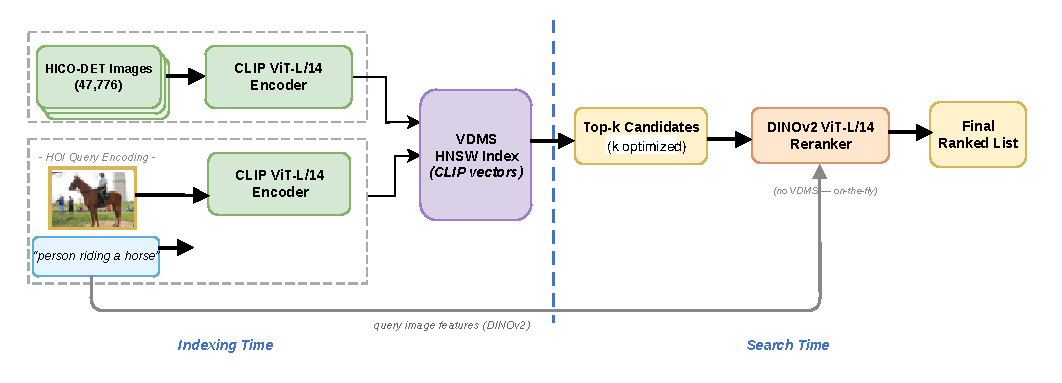
\includegraphics[width=\textwidth]{figures/pipeline_figure.pdf}
  \caption{Two-stage HOI retrieval pipeline.
    Stage~1: a CLIP ViT-L/14 text embedding drives ANN search in VDMS,
    returning a top-$k$ candidate pool via a configurable ANN index
    (FaissFlat, FaissHNSWFlat, or FaissIVFFlat).
    Stage~2: DINOv2 ViT-L/14-reg4 visual distances rerank the pool
    on-the-fly via weighted score fusion --- no additional index is required
    at deployment.}
  \label{fig:pipeline}
\end{figure*}

\subsection{Overview}

Let $\mathcal{C} = \{(\mathbf{c}_i,\,\mathbf{d}_i)\}_{i=1}^{N}$ denote the corpus
of $N{=}47{,}776$ images, where $\mathbf{c}_i \in \mathbb{R}^{768}$ is the
unit-normalized CLIP ViT-L/14 embedding and $\mathbf{d}_i \in \mathbb{R}^{1024}$
is the unit-normalized DINOv2 ViT-L/14-reg4 embedding of image $i$.
For HOI class $h$, let $\mathcal{I}_h \subseteq [N]$ denote the annotated relevant
image set.
Given a text query $q$ (e.g., \textit{``a person riding a horse''}), the pipeline
proceeds in two stages, as illustrated in Figure~\ref{fig:pipeline}.

\textbf{Stage~1} encodes $q$ into a 768-dimensional unit-norm query vector
$\mathbf{q}_c \in \mathbb{R}^{768}$ using the CLIP ViT-L/14 text encoder and
issues an ANN search over the VDMS CLIP DescriptorSet to retrieve a top-$k$ candidate
pool $\mathcal{T}_k(q)$.
\textbf{Stage~2} reranks $\mathcal{T}_k(q)$ using DINOv2 visual distances without
requiring any additional index: a per-class reference vector $\mathbf{r}_h$ is
computed once at initialization from the DINOv2 embeddings of a small representative
subset of $\mathcal{I}_h$, and the CLIP and DINOv2 distances of each candidate are
fused into a single score.
The five configuration parameters $\{$engine, $M$ or \textit{nlist}, \textit{efSearch}
or \textit{nprobe}, $k$, $\alpha\}$ jointly govern the accuracy--throughput trade-off
and are selected by the LLM optimizer described in Section~\ref{sec:optimizer}.

\subsection{Stage 1: CLIP-Based ANN Retrieval}

All 47{,}776 CLIP ViT-L/14 image embeddings are pre-computed offline using the OpenAI
weights and stored in VDMS as a 768-dimensional L2 DescriptorSet.
At query time, $q$ is encoded by the frozen CLIP text encoder and the resulting
$\mathbf{q}_c$ is submitted to VDMS as a \texttt{FindDescriptor} request.
VDMS returns the top-$k$ candidate identifiers with their L2 distances
$\delta_j^c = \|\mathbf{c}_j - \mathbf{q}_c\|_2$; the candidate pool is formally
\begin{equation}
  \mathcal{T}_k(q) = \bigl\{j \in [N] : \|\mathbf{c}_j - \mathbf{q}_c\|_2 \leq \delta^{(k)}\bigr\} ,
  \label{eq:stage1}
\end{equation}
where $\delta^{(k)}$ is the $k$-th smallest L2 distance to $\mathbf{q}_c$ across the full corpus.
For FaissFlat this set is exact; for FaissHNSWFlat and FaissIVFFlat, VDMS returns a
high-recall approximation.
Three ANN engines are available, each exposing a different accuracy--throughput
operating point:
\begin{itemize}[noitemsep,topsep=2pt]
  \item \textbf{FaissFlat}: exact exhaustive search; highest recall, lowest QPS.
  \item \textbf{FaissHNSWFlat}~\cite{malkov2018hnsw}: graph-based ANN index;
    accuracy controlled by graph connectivity $M \in \{8, 16, 32, 48, 64\}$
    and search beam width $\mathit{efSearch} \in \{32, 64, 100, 150, 200, 300, 500\}$.
  \item \textbf{FaissIVFFlat}~\cite{johnson2019billion}: inverted-file ANN index;
    accuracy controlled by $\mathit{nlist} \in \{64, 128, 256, 512\}$ clusters
    and $\mathit{nprobe} \in \{4, 8, 16, 32, 64\}$ probed clusters.
\end{itemize}
Increasing $k$ improves Stage~2 recall at the cost of higher reranking latency;
the optimal $k \in \{50, 100, 150, 200, 300, 500, 750, 1000\}$ is jointly selected
with the engine parameters.

\subsection{Stage 2: DINOv2 Reranking}

\noindent\textbf{Reference vector.}
DINOv2 ViT-L/14-reg4 is a self-supervised visual encoder that captures fine-grained
appearance features --- object identity, texture, and spatial structure ---
complementary to CLIP's language-aligned semantic embeddings.
We represent each HOI class $h$ by a reference vector
$\mathbf{r}_h \in \mathbb{R}^{1024}$, computed once at initialization as the mean
DINOv2 embedding of a selected subset $\mathcal{S}_h \subseteq \mathcal{I}_h$ of
$n_r \in \{1, 3, 5, 10\}$ images:
\begin{equation}
  \mathbf{r}_h \;=\; \frac{1}{n_r} \sum_{i \in \mathcal{S}_h} \mathbf{d}_i .
  \label{eq:refvec}
\end{equation}
Three strategies select $\mathcal{S}_h$: \textbf{first} takes the first $n_r$ images
in dataset order; \textbf{centroid} selects the $n_r$ images closest to the class mean
$\boldsymbol{\mu}_h^d = \frac{1}{|\mathcal{I}_h|}\sum_{i \in \mathcal{I}_h}\mathbf{d}_i$;
\textbf{diverse} applies greedy farthest-point sampling, seeding from the most central
image and iteratively adding the image furthest from the already-selected set to maximize
intra-subset spread.
Reference vector construction is a one-time cost ($<$1\,ms per class in numpy) and
imposes no per-query overhead.

\noindent\textbf{Distance normalization.}
CLIP and DINOv2 distances operate at different absolute scales and cannot be directly
combined.
We apply min-max normalization \emph{within} $\mathcal{T}_k(q)$ to map both onto
$[0,\,1]$:
\begin{equation}
  \hat{c}_j =
    \frac{\delta_j^c - \min_{i \in \mathcal{T}_k}\delta_i^c}
         {\max_{i \in \mathcal{T}_k}\delta_i^c
          - \min_{i \in \mathcal{T}_k}\delta_i^c + \varepsilon} ,
  \label{eq:clipnorm}
\end{equation}
\begin{equation}
  \hat{d}_j =
    \frac{\delta_j^d - \min_{i \in \mathcal{T}_k}\delta_i^d}
         {\max_{i \in \mathcal{T}_k}\delta_i^d
          - \min_{i \in \mathcal{T}_k}\delta_i^d + \varepsilon} ,
  \label{eq:dinonorm}
\end{equation}
where $\delta_j^d = \|\mathbf{d}_j - \mathbf{r}_h\|_2$ is the DINOv2 distance of
candidate $j$ to the class reference vector and $\varepsilon = 10^{-10}$ prevents
division by zero.
Normalizing within the candidate pool --- rather than globally across the corpus ---
ensures the two scores remain commensurate regardless of the per-query scale of
retrieved distances.

\noindent\textbf{Fusion and final ranking.}
The fusion score for candidate $j \in \mathcal{T}_k(q)$ is the convex combination
\begin{equation}
  s_j \;=\; (1-\alpha)\,\hat{c}_j \;+\; \alpha\,\hat{d}_j ,
  \label{eq:fusion}
\end{equation}
where $\alpha \in \{0.0, 0.05, \ldots, 0.90\}$ governs the DINOv2 contribution.
Lower $s_j$ indicates higher relevance.
The final ranked list is $\mathcal{T}_k(q)$ sorted by $s_j$ in ascending order.
Setting $\alpha{=}0$ reduces the system to CLIP-only ranking; $\alpha{=}1$ reduces it
to DINOv2-only ranking.
The optimal $\alpha$ is data-dependent and is selected jointly with the ANN engine
configuration by the optimizer in Section~\ref{sec:optimizer}.

\subsection{Why Text Queries Outperform Image Queries: Centroid Geometry}

We formalize why a text query systematically outperforms a single reference image on
compositionally structured HOI categories, grounding the argument in the geometry of
CLIP's joint embedding space.

Let $\boldsymbol{\mu}_h^c = \frac{1}{|\mathcal{I}_h|}\sum_{i\in\mathcal{I}_h}\mathbf{c}_i$
denote the visual centroid of class $h$ in CLIP space, and let
$\sigma_h^2 = \frac{1}{|\mathcal{I}_h|}\sum_{i \in \mathcal{I}_h}
\|\mathbf{c}_i - \boldsymbol{\mu}_h^c\|_2^2$ be the intra-class variance.
For any query vector $\mathbf{q}' \in \mathbb{R}^{768}$, the bias--variance
decomposition of the expected squared L2 distance to a uniformly sampled class
member $\mathbf{c}_i$ ($i \sim \mathcal{I}_h$) is:
\begin{equation}
  \mathbb{E}_{i}\bigl[\|\mathbf{q}' - \mathbf{c}_i\|_2^2\bigr]
  \;=\;
  \underbrace{\|\mathbf{q}' - \boldsymbol{\mu}_h^c\|_2^2}_{\text{bias}^2}
  \;+\;
  \underbrace{\sigma_h^2}_{\text{variance}} .
  \label{eq:biasvar}
\end{equation}
The variance term $\sigma_h^2$ is fixed by the data; only the bias term
$\|\mathbf{q}' - \boldsymbol{\mu}_h^c\|_2^2$ depends on the choice of query.

CLIP's contrastive training aligns the text embedding of a category description with the
visual embeddings of matching images~\cite{radford2021clip}.
For a compositionally structured category such as \textit{``a person riding a horse''} ---
which spans diverse viewpoints, backgrounds, and subjects --- the text embedding aggregates
signals from many matched images and therefore lies near the visual centroid of the class:
$\mathbf{q}_c \approx \boldsymbol{\mu}_h^c$, making the bias term in
Eq.~\eqref{eq:biasvar} approximately zero:
\begin{equation}
  \mathbb{E}_{i}\bigl[\|\mathbf{q}_c - \mathbf{c}_i\|_2^2\bigr]
  \;\approx\; \sigma_h^2 .
  \label{eq:textquery}
\end{equation}
In contrast, a reference image $\mathbf{c}_j$ ($j \in \mathcal{I}_h$) lies at
displacement $\varepsilon_j = \|\mathbf{c}_j - \boldsymbol{\mu}_h^c\|_2 > 0$ from
the centroid, contributing a positive bias term:
\begin{equation}
  \mathbb{E}_{i}\bigl[\|\mathbf{c}_j - \mathbf{c}_i\|_2^2\bigr]
  \;=\; \varepsilon_j^2 + \sigma_h^2
  \;>\; \sigma_h^2 .
  \label{eq:imagequery}
\end{equation}
The text query therefore achieves lower expected squared distance to every class member
than any individual reference image, by a margin of $\varepsilon_j^2$.
This advantage is largest for visually diverse categories: for an HOI class spanning many
viewpoints and subjects (e.g., \textit{ride horse}), any single reference image lies far
from the centroid ($\varepsilon_j$ large) and provides a poor proxy for the full category
distribution, amplifying the margin over a text query.
Under L2-based ANN retrieval, lower expected distance to class members translates
directly to higher recall at any fixed $k$, and therefore to higher mAP.

\section{LLM-Guided ANN Hyperparameter Optimization}
\label{sec:optimizer}

Figure~\ref{fig:workflow} illustrates the overall optimization framework.
Four methods --- LLM Agent, Optuna TPE, Grid Search, and Random Search --- each propose
a joint index configuration (engine, $M$, \textit{efSearch}/\textit{nlist}/\textit{nprobe},
pool size $k$, fusion weight $\alpha$, reference count $n_r$, reference strategy) over $N=30$ iterations.
Each proposed configuration is loaded into a VDMS Apptainer container, which builds the
ANN index and executes all 600 HICO-DET queries; the resulting mAP and QPS are
combined into Score $= \text{mAP} \times \text{QPS}$ (HICO-DET) or
$\text{QPS} \times \text{Recall@10}$ (SIFT1M).
Only adaptive methods --- the LLM Agent and Optuna TPE --- receive the score signal as
feedback to inform subsequent proposals; Grid Search and Random Search are non-adaptive
baselines that do not condition on observed outcomes.

\begin{figure*}[t]
  \centering
  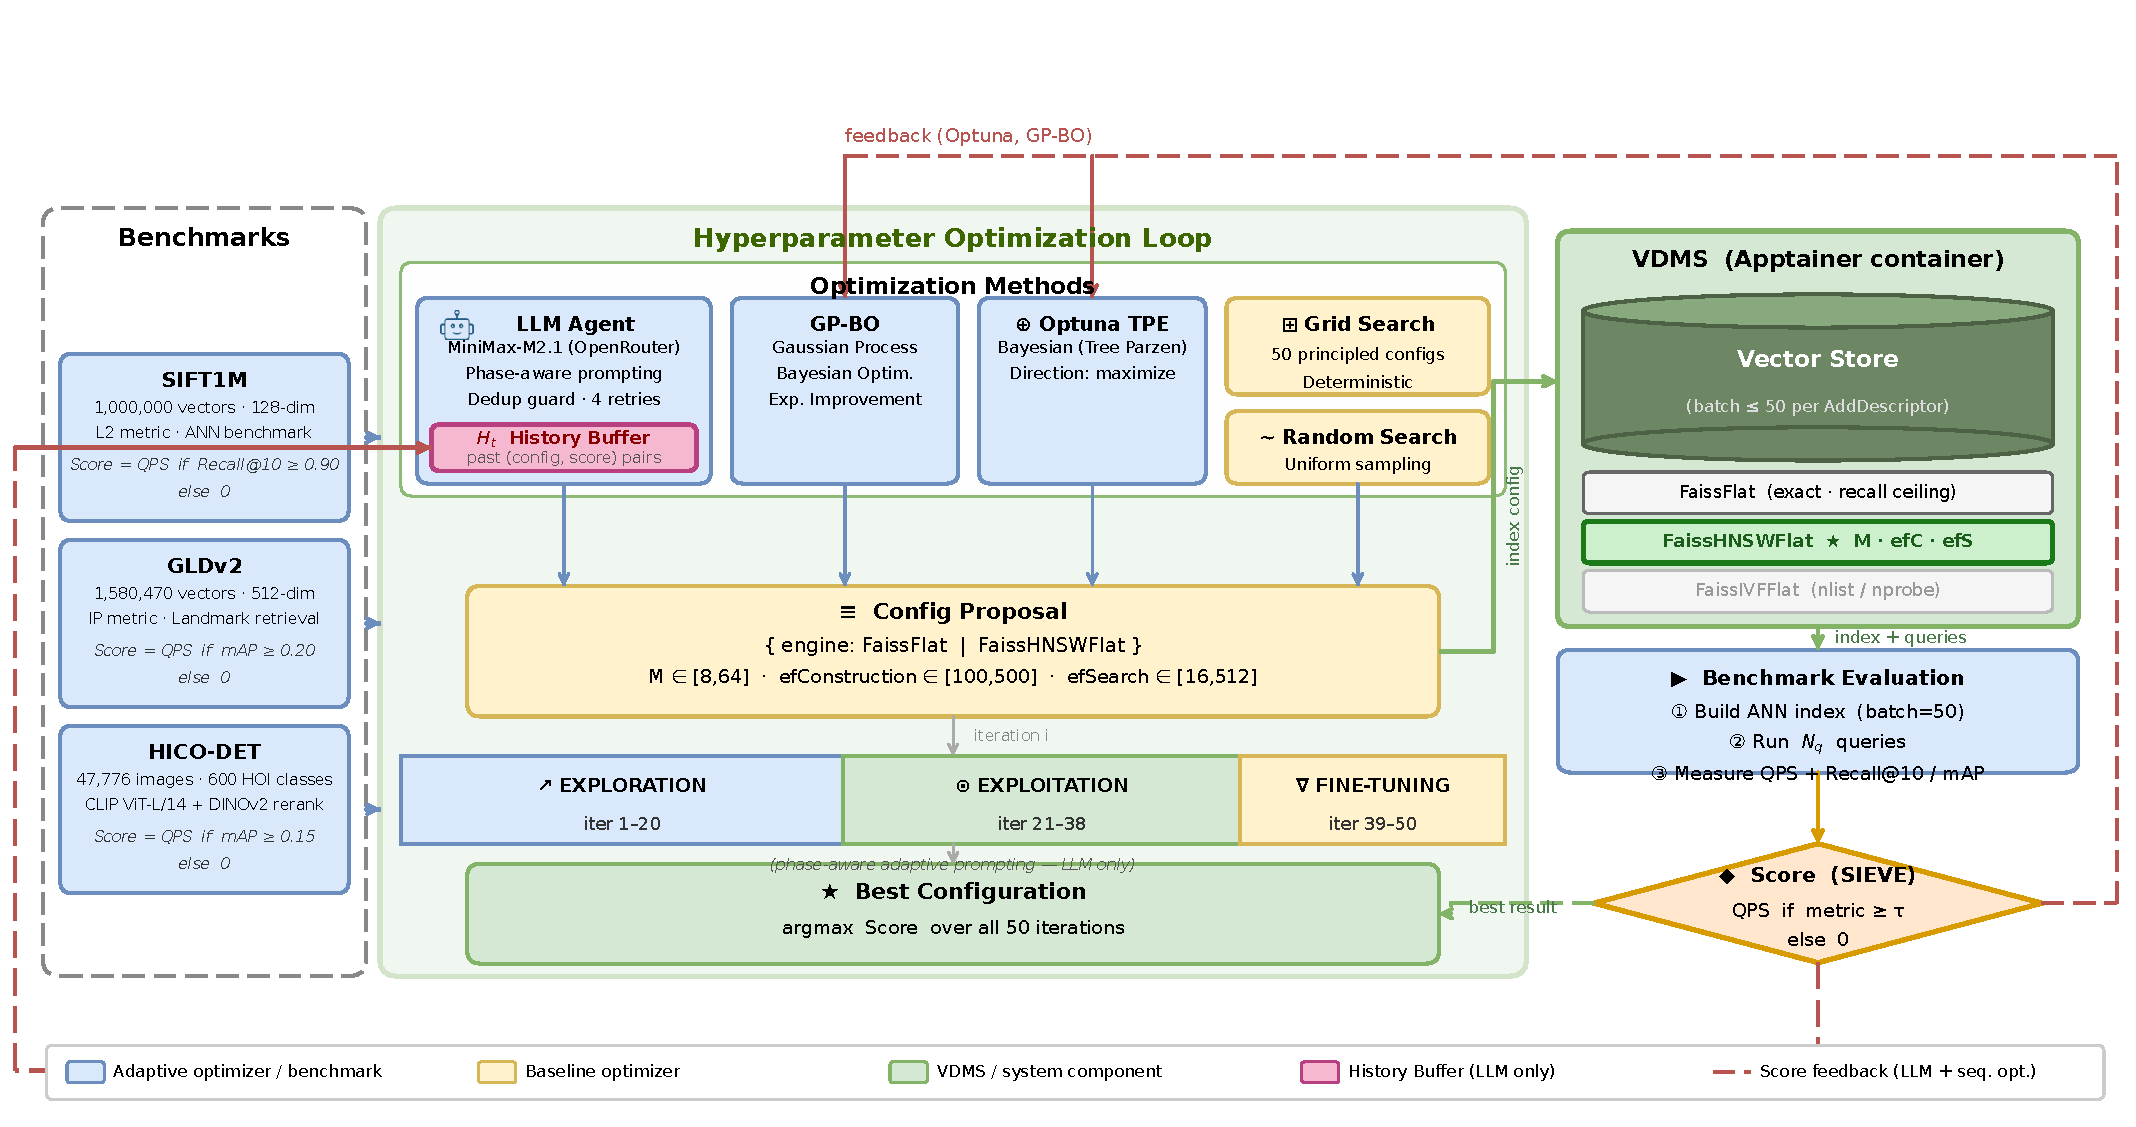
\includegraphics[width=\textwidth]{figures/workflow.pdf}
  \caption{Overview of the Agentic VDMS optimization framework.
    Four methods --- \textbf{LLM Agent} (phase-aware, adaptive) and \textbf{Optuna TPE}
    (Bayesian, adaptive) vs.\ \textbf{Grid Search} and \textbf{Random Search}
    (non-adaptive baselines) --- each propose ANN index configurations evaluated by VDMS
    over $N{=}30$ iterations.
    Score $= \text{QPS} \times \text{Recall@10}$ (SIFT1M) or
    $\text{mAP} \times \text{QPS}$ (HICO-DET).
    Red dashed arrows indicate score feedback; only adaptive methods receive it.}
  \label{fig:workflow}
\end{figure*}

\begin{figure*}[t]
  \centering
  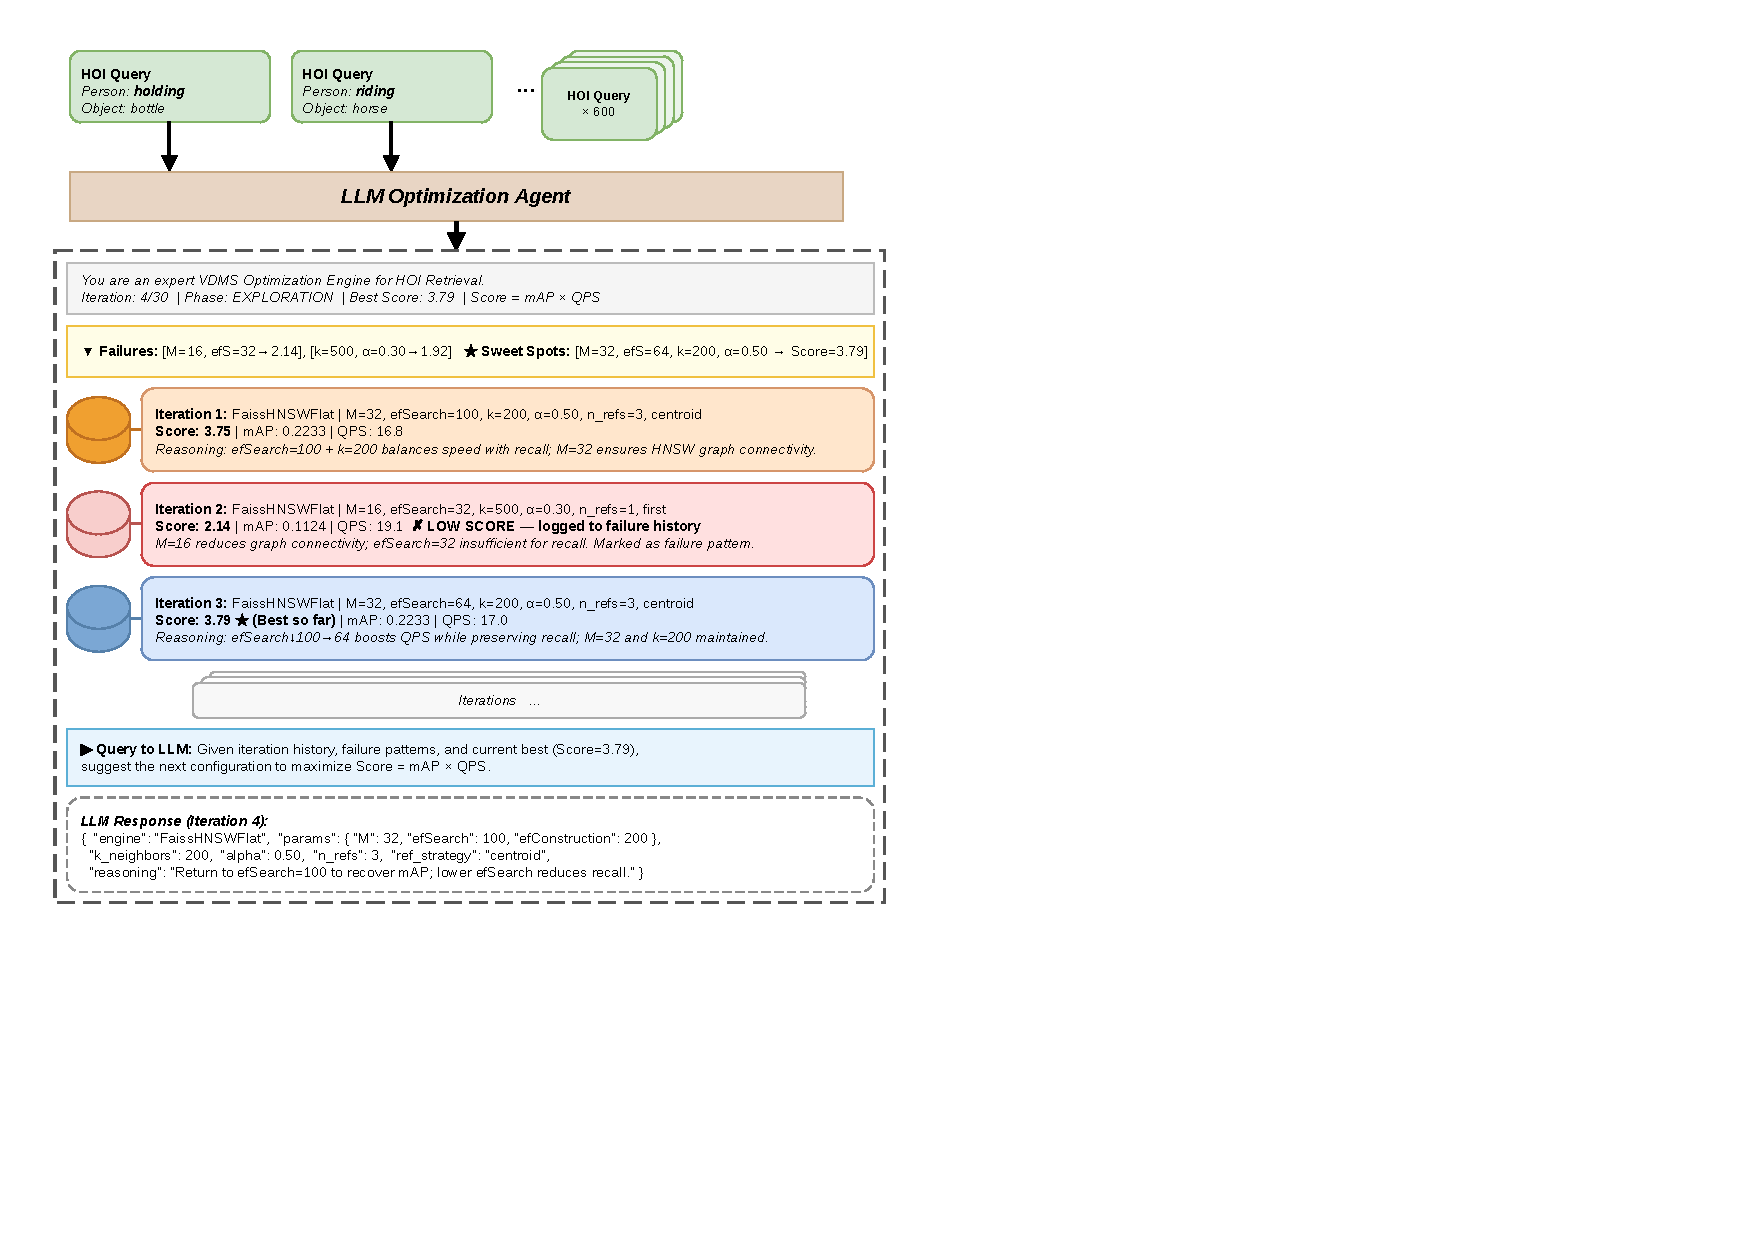
\includegraphics[width=\textwidth]{figures/prompts.pdf}
  \caption{LLM prompt structure used by the agent for ANN index hyperparameter
    optimization. The system prompt establishes the optimization objective;
    the user prompt supplies the measured Score history and asks the agent to
    propose the next configuration.}
  \label{fig:prompts}
\end{figure*}

\subsection{Agent Design}

The LLM agent operates as a closed-loop optimizer over a mixed-type search space of
approximately $102{,}000$ configurations, defined by three engines with
engine-conditional parameters ($M \in \{8,16,32,48,64\}$ and
$\mathit{efSearch} \in \{32,64,100,150,200,300,500\}$ for FaissHNSWFlat;
$\mathit{nlist} \in \{64,128,256,512\}$ and $\mathit{nprobe} \in \{4,8,16,32,64\}$
for FaissIVFFlat), pool size $k \in \{50,\ldots,1000\}$, fusion weight
$\alpha \in \{0.0, 0.05, \ldots, 0.90\}$, reference count
$n_r \in \{1,3,5,10\}$, and reference strategy $\in \{\text{first, centroid, diverse}\}$.

\smallskip
\noindent\textbf{Prompt structure.}
At each iteration $t$, the agent receives a single prompt containing:
(i) a description of the VDMS two-stage pipeline architecture and per-engine parameter
physics --- including the known dependency that $\mathit{efSearch}$ and $M$ must be
co-tuned, and that \textit{efSearch} $\ll k$ accepts ANN approximation error in exchange
for throughput;
(ii) a \emph{per-iteration diagnostic} derived from the observed Score relative to the
running best, selecting one of five feedback classes
(\textit{excellent}, \textit{explore\_more}, \textit{low\_mAP}, \textit{low\_QPS},
or \textit{moderate}) and providing targeted guidance on which parameter axis to adjust;
(iii) the complete ordered history of all $t{-}1$ evaluated
(configuration, Score, mAP, QPS) tuples;
(iv) a dynamically computed list of untried $\alpha$ values and untried
$(n_r, \text{ref\_strategy})$ pairs, derived at inference time from the history;
and (v) seven decision rules governing structural diversity, stagnation escape, and
an anti-collapse constraint that prohibits consecutive iterations that vary only
$\alpha$ without any structural change.
The agent responds with a structured JSON object specifying the next configuration
and a \textit{reasoning} field articulating its rationale.
Figure~\ref{fig:prompts} illustrates the prompt template.

\smallskip
\noindent\textbf{Phase-aware strategy.}
The $N$-iteration budget is partitioned into three phases whose boundaries scale with $N$:
\textbf{Exploration} (iterations $1$--$\lfloor 0.4N \rfloor$) broadly varies engine,
$M$, and $k$ across structurally distinct regions to map the Score landscape;
\textbf{Exploitation} (iterations $\lfloor 0.4N \rfloor{+}1$--$\lfloor 0.75N \rfloor$)
refines the most promising engine--$M$ combination found during exploration, focusing
on $\alpha$, $n_r$, and reference strategy;
and \textbf{Fine-tuning} (iterations $\lfloor 0.75N \rfloor{+}1$--$N$) performs
narrow coordinate refinement of $\alpha$ and reference strategy around the current best.
This schedule encodes the domain insight that structural choices (engine, $M$) determine
the achievable QPS ceiling and must be resolved before continuous choices ($\alpha$, $n_r$)
are optimized --- a conditional dependency between parameters that Optuna TPE, which models
each parameter independently via univariate kernel density estimation, cannot exploit.

\smallskip
\noindent\textbf{Duplicate avoidance.}
Each proposal is checked against the complete evaluation history.
If a duplicate configuration is detected, the prompt is resubmitted with an explicit
rejection notice listing the already-evaluated configuration and its score.
Up to four retries are attempted; after four consecutive duplicates, a uniformly random
valid configuration is selected as a fallback, ensuring the optimization loop continues
without stalling.

\section{Experiments}
\label{sec:experiments}

\subsection{Experimental Setup}

\noindent\textbf{Dataset.}
We evaluate on the HICO-DET retrieval benchmark introduced in
Section~\ref{sec:benchmark}: 47{,}776 images, 600 text queries, and 90{,}641
ground-truth positive pairs.
All image embeddings are 768-dimensional CLIP ViT-L/14 vectors stored in VDMS.

\noindent\textbf{Compared Methods.}
We compare four optimization strategies, each run for $N{=}30$ iterations:
\begin{itemize}[noitemsep,topsep=2pt]
  \item \textbf{LLM Agent (Ours):} at each iteration, the agent receives the full
    history of (configuration, Score) pairs in its prompt and proposes the next
    configuration; implemented with MiniMax-M2.1 via OpenRouter.
  \item \textbf{Optuna TPE}~\cite{akiba2019optuna}: Tree-structured Parzen Estimator
    Bayesian optimization; adaptive, conditions on observed outcomes.
  \item \textbf{Random Search}~\cite{bergstra2012random}: samples configurations
    uniformly at random; non-adaptive.
  \item \textbf{Grid Search}: enumerates a fixed grid of configurations in
    lexicographic order; non-adaptive.
\end{itemize}
As system baselines we include UniIR~\cite{wei2023uniir} (CLIP ViT-L/14, brute-force),
standalone CLIP ViT-L/14 (FaissFlat), standalone DINOv2 ViT-L/14-reg4 (FaissFlat), and
CLIP$+$DINOv2 reranking (FaissFlat), all using exact search to establish
accuracy upper bounds independent of ANN approximation.

\noindent\textbf{Metrics.}
Retrieval quality is measured by mean Average Precision at $k{=}10$ (mAP@10), the
standard metric for ranked retrieval with multiple relevant documents~\cite{manning2008ir},
as well as Precision@10, NDCG@10, and Recall@10.
Throughput is measured in queries per second (QPS), averaged over all 600 queries issued
as a single batch.
The joint optimization objective is Score $= \text{mAP} \times \text{QPS}$.

\noindent\textbf{Implementation.}
All experiments run on the NCSA Delta cluster (partition \texttt{gpuA40x4}): one
NVIDIA A40 GPU, 16 CPU cores (AMD EPYC 7763), and exclusive node access.
VDMS is deployed as an Apptainer container; all retrieval and optimization code is
implemented in Python~3.12.
For Optuna, we use the official \texttt{optuna} library~\cite{akiba2019optuna} with the
default TPE sampler.
Each iteration builds a full ANN index and issues 600 queries, taking approximately
7--8 minutes of wall-clock time.

\begin{figure*}[t]
  \centering
  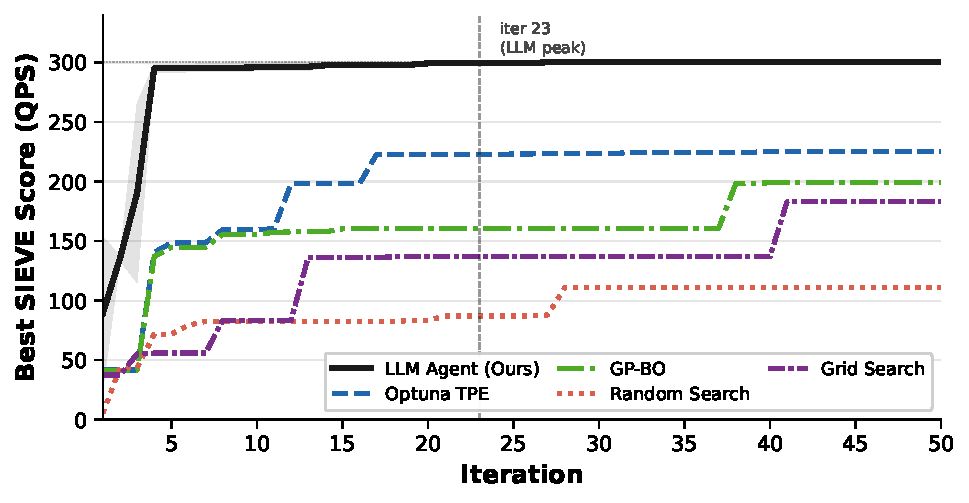
\includegraphics[width=\textwidth]{figures/convergence_hico_det.pdf}
  \caption{Convergence of optimization methods on HICO-DET over 30 iterations.
    Best Score ($\text{mAP} \times \text{QPS}$) achieved so far is plotted at
    each iteration.
    The LLM agent reaches Score $= 3.86$ by iteration~5 --- a level that
    Optuna TPE first matches at iteration~9 and Random Search first matches at
    iteration~28 --- and continues improving to Score $= 4.34$ at iteration~30
    through its phase-aware exploitation strategy.
    Grid Search early-stops at iteration~12 after failing to improve for five
    consecutive iterations.}
  \label{fig:convergence}
\end{figure*}

\subsection{System Baselines}

Table~\ref{tab:baselines} characterizes three fundamental properties of the benchmark.
\textbf{Compositional difficulty:} even exact-search CLIP$+$DINOv2 achieves only
mAP $= 0.276$, because fine-grained HOI categories share the same object class but
differ only in action verb (e.g., \textit{ride}, \textit{sit\_on}, and \textit{straddle}
applied to horse); CLIP's shared embedding space partially conflates these categories,
making high mAP structurally hard to achieve.
\textbf{Modality gap:} DINOv2 alone (mAP $= 0.217$, Score $= 0.250$) underperforms
CLIP alone at equal $k{=}2000$ (mAP $= 0.240$, Score $= 0.280$), confirming
that semantic language alignment is essential for compositional HOI retrieval and that
visual appearance alone is insufficient.
\textbf{ANN efficiency vs accuracy:} reducing $k$ from 2000 to 500 in CLIP-only
retrieval raises QPS by $7.0\times$ (8.21 vs.\ 1.17) and Score by $6.1\times$
(1.707 vs.\ 0.280), but costs 3.2 percentage points of mAP (0.208 vs.\ 0.240),
illustrating the sharp accuracy--throughput trade-off that Score $= \text{mAP} \times \text{QPS}$
is designed to navigate jointly.

\subsection{Optimizer Comparison and Sample Efficiency}

% ── Table 2: Optimizer comparison ─────────────────────────────────────────────
\begin{table*}[t]
\centering
\caption{Comparison of ANN index hyperparameter optimization methods on HICO-DET (30 iterations, best config reported).
  Score $= \text{mAP} \times \text{QPS}$.
  Build: index construction time. CLIP / DINOv2: per-query inference time.
  \emph{Iters$\to$Best}: first iteration achieving the best score.
  $\dagger$~Grid Search early-stopped at iteration 12 (patience$=$5).
  The LLM agent achieves the highest Score and reaches competitive performance within 5 iterations --- a level requiring 9 iterations for Optuna TPE and 28 for Random Search.}
\label{tab:optimizer}
\footnotesize
\setlength{\tabcolsep}{4.5pt}
\begin{tabular}{lccccccccccc}
\toprule
\textbf{Method} & \textbf{Score}$\uparrow$ & \textbf{mAP}$\uparrow$ & \textbf{P@10}$\uparrow$ & \textbf{NDCG@10}$\uparrow$ & \textbf{R@10}$\uparrow$ & \textbf{QPS}$\uparrow$ & \textbf{Build (s)}$\downarrow$ & \textbf{CLIP (ms)}$\downarrow$ & \textbf{DINOv2 (ms)}$\downarrow$ & \textbf{Total Lat.\ (ms)}$\downarrow$ & \textbf{Iters$\to$Best} \\
\midrule
Grid Search$^\dagger$
  & 3.027 & 0.148 & ---   & ---    & ---    & 20.49 & $\sim$445 & --- & --- & --- & 7/12 \\
Random Search
  & 4.095 & 0.200 & 0.449 & 0.509  & 0.148  & 20.47 & 444.3 & 48.3 & 0.32 & 48.9 & 28/30 \\
Optuna TPE
  & 4.113 & 0.258 & 0.502 & 0.572  & 0.178  & 15.97 & 423.3 & 62.0 & 0.47 & 62.6 & 27/30 \\
\textbf{LLM Agent (Ours)}
  & \textbf{4.337} & 0.255 & 0.489 & 0.564 & 0.168 & \textbf{16.98} & 441.8 & \textbf{58.2} & \textbf{0.49} & \textbf{58.9} & \textbf{30/30} \\
\bottomrule
\end{tabular}
\end{table*}

\noindent\textbf{Overall performance.}
Table~\ref{tab:optimizer} and Figure~\ref{fig:convergence} report the results of all four
optimization methods over 30 iterations.
The LLM agent achieves the highest Score $= 4.337$, a $\mathbf{2.5\times}$ improvement
over the CLIP FaissFlat baseline (Score $= 1.707$) and $\mathbf{13.6\times}$ over
brute-force CLIP$+$DINOv2 reranking (Score $= 0.319$).
At its optimal configuration --- FaissHNSWFlat with $M{=}48$,
$\mathit{efSearch}{=}64$, $k{=}200$, $\alpha{=}0.80$, $n_r{=}10$,
and \textit{centroid} reference selection --- the pipeline achieves
mAP $= 0.255$ and QPS $= 16.98$, representing a $14.7\times$ throughput gain
over brute-force CLIP$+$DINOv2 (QPS $= 1.15$) at a cost of only 2.1 percentage points
of mAP (0.255 vs.\ 0.276).
Optuna TPE (Score $= 4.113$) and Random Search (Score $= 4.095$) reach comparable final
scores, both trailing the LLM agent by approximately 5--6\%.
Grid Search (Score $= 3.027$) performs substantially worse, early-stopping at
iteration~12 after failing to improve for five consecutive iterations.

\smallskip
\noindent\textbf{Sample efficiency.}
The LLM agent's key advantage is \emph{sample efficiency}: it reaches Score $= 3.86$
by iteration~5, already exceeding Grid Search's final best (Score $= 3.027$) and
surpassing both Optuna TPE (Score $= 3.142$ at iteration~10) and Random Search
(Score $= 2.294$ at iteration~10).
Optuna TPE first exceeds the LLM agent's iteration-5 performance at iteration~9
(Score $= 3.905$); Random Search does not match it until iteration~28 (Score $= 4.095$).
At ${\approx}7$--$8$ minutes of wall-clock time per evaluation, this translates
to concrete savings: the LLM agent reaches Score~$\geq 3.86$ roughly 30 minutes
before Optuna TPE (four fewer evaluations) and over 2.5 hours before Random Search
(23 fewer evaluations).
This sample efficiency directly follows from the agent conditioning each new proposal
on the full empirical history, rather than sampling blindly or relying on parameter-independent
density estimates.

\smallskip
\noindent\textbf{Configuration insight.}
The optimal configuration discovered by the LLM agent reveals a non-obvious accuracy--throughput
operating point.
The agent sets $\mathit{efSearch}{=}64$ --- well below the conventional HNSW heuristic
of $\mathit{efSearch} \geq k$~\cite{malkov2018hnsw} --- accepting higher ANN approximation
error in exchange for greater query throughput.
This approximation is compensated downstream by the DINOv2 reranker with $\alpha{=}0.80$,
which reassigns 80\% of the final score weight to visual similarity over the
top-$k{=}200$ pool.
The agent further discovers that $n_r{=}10$ centrally-selected reference images
substantially outperform $n_r{=}1$: the mean DINOv2 embedding of ten images nearest
the class centroid is a far more stable proxy for the HOI class distribution than any
single image, reducing the bias term $\varepsilon_j^2$ in Eq.~\eqref{eq:imagequery}.
This three-way interaction among $\mathit{efSearch}$, $k$, and $\alpha$ is the key
region that non-adaptive baselines fail to locate.

\smallskip
\noindent\textbf{Failure modes of non-adaptive methods.}
Grid Search's poor performance is a direct consequence of its one-dimensional sweep
design: it sweeps $k$ while holding $M{=}32$ and $\alpha{=}0.30$ fixed, never
testing $M{=}48$ (the LLM's optimal value) and never exploring $\alpha > 0.30$
(vs.\ the optimal $\alpha{=}0.80$).
The lexicographic enumeration order ensures that the joint optimum of
$(M, k, \alpha, n_r, \text{ref\_strategy})$ is never evaluated.
Optuna TPE exhibits premature convergence: at iterations~11--13, all three evaluations
produce configurations with identical mAP $= 0.169$ and QPS $= 18.6$, reflecting
the difficulty of TPE's univariate density estimator on a search space with hard
structural dependencies between engine type and its valid parameters.
The TPE sampler, lacking any representation of the conditional relationship between
engine and its hyperparameters, wastes evaluations on repeatedly sampling
the same low-scoring FaissIVFFlat region before eventually discovering the optimal
configuration at iteration~27.

\section{Conclusion}
\label{sec:conclusion}

% TODO: fill in conclusion

\begin{acks}
 This work was supported by the [...] Research Fund of [...] (Number [...]). Additional funding was provided by [...] and [...]. We also thank [...] for contributing [...].
\end{acks}

\clearpage

\bibliographystyle{ACM-Reference-Format}
\bibliography{sample}

\end{document}
\endinput
